\section{Background and Problem}

%$$$$$$$$$$$$$$$$$$$$$$$$$$$$$$$$$$$$$$$$$$$$$$$$$$$$$$$$$$$$$$$$$$$$$$$$$$$$$$$$
% Paragraph : Linux Scalability : Fork intensive workload 문제점 설명 
%$$$$$$$$$$$$$$$$$$$$$$$$$$$$$$$$$$$$$$$$$$$$$$$$$$$$$$$$$$$$$$$$$$$$$$$$$$$$$$$$

\begin{figure}
  \begin{subfigure}[b]{0.23\textwidth}
    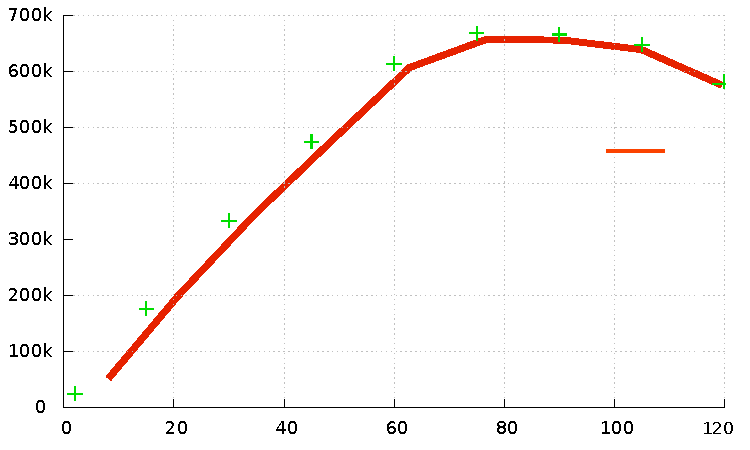
\includegraphics[width=\textwidth]{graph/aim7_default}
    \caption{AIM7-multiuser scalability}
  \end{subfigure}%
  \begin{subfigure}[b]{0.25\textwidth}
    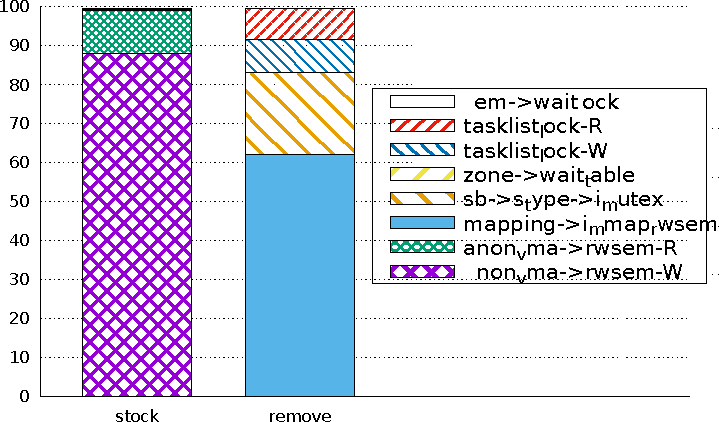
\includegraphics[width=\textwidth]{graph/lockstat}
    \caption{Lock profile on 120core}
  \end{subfigure}
  \centering
  \footnotesize {
  \caption{Scalability of AIM7 multiuser and lock waiting time on 120core.
  This workload simultaneously create many processes. The (a) shows up to 75
  core, the stock Linux scale linearly, then they flattens out. The (b)
  represents anonymous r/w lock is , and file mapping r/w is scalability
  bottleneck}
  \label{fig:aim7_default} }
\end{figure}

Applications performance would be limited by the operating system when the
operating system does not scale~\cite{Clements15SCR}[Corey].
Linux has heavily optimized for multi-core operating systems, so we examine
AIM7-multiuser benchmark on the Linux.
The AIM benchmark has, until recently, been widely used in research area
and Linux community~\cite{Bueso2015STP}~\cite{Bueso2014MCS}.
This AIM7-multiuser workload simultaneously creates many processes with
disk-file operations, virtual memory operations, pipe I/O, and arithmetic
operation, and we uses the temp filesystem to minimize the file system
bottleneck.
The results of scalability shows the stock Linux scales linearly up to 60 core,
then they flattens out(Figure xx(a)).

%$$$$$$$$$$$$$$$$$$$$$$$$$$$$$$$$$$$$$$$$$$$$$$$$$$$$$$$$$$$$$$$$$$$$$$$$$$$$$$$$
% Paragraph: Lockstat로 분석 결과 설명 
%$$$$$$$$$$$$$$$$$$$$$$$$$$$$$$$$$$$$$$$$$$$$$$$$$$$$$$$$$$$$$$$$$$$$$$$$$$$$$$$$

To understand the source of scalability bottleneck on 120core, we profile a lock
contention using the lock\_stat[], a Linux kernel lock profiler that reports how
long each lock is held and the wait time to acquire the lock.
The Figure-xx (b) show the cost of acquiring the lock when the AIM7-multiuser
runs on the 120 core the Linux machine.
As the result of the lock\_stat, the main problem of lock contention is the
anonymous reverse mapping reader-writer semaphore(anon\_vma->rwsem).
, which is generated by simultaneously creating a number of process.
The reverse page mapping records page information when using fork(), exit() and
mmap() system call to find all page table entries.
To understand the other bottleneck, we conducted a workaround by removing
anonymous rmap relative code in the part of the fork code with page-swap off
avoiding the Linux page reclaiming.
When the anon\_vma is removed, the Linux is contended on file reverse page
mapping(i\_mmaping-rwsem).

%$$$$$$$$$$$$$$$$$$$$$$$$$$$$$$$$$$$$$$$$$$$$$$$$$$$$$$$$$$$$$$$$$$$$$$$$$$$$$$$$
% Paragraph : 리눅스 reverse page map의 write serialization 문제점
%$$$$$$$$$$$$$$$$$$$$$$$$$$$$$$$$$$$$$$$$$$$$$$$$$$$$$$$$$$$$$$$$$$$$$$$$$$$$$$$$

Our research recognized both the anonymous reverse page mapping
reporting from Linux community[] and the file reverse page mapping reporting from S.
Boyd-Wickizer[] are a significant factor in a fork scalability problem.
Thus, in order to perfect scalability of the fork, both the
file reverse mapping and the anonymous reverse mapping should be executed
concurrently without lock.
In other words, the fundamental scalability problem of reverse mapping is their
serialized updates operation because operating system kernel are serialized at
the updates operation.

%$$$$$$$$$$$$$$$$$$$$$$$$$$$$$$$$$$$$$$$$$$$$$$$$$$$$$$$$$$$$$$$$$$$$$$$$$$$$$$$$
% Paragraph : update heavy한 상황에 대한 설명과 해결 방법에 대한 설명
%$$$$$$$$$$$$$$$$$$$$$$$$$$$$$$$$$$$$$$$$$$$$$$$$$$$$$$$$$$$$$$$$$$$$$$$$$$$$$$$$

In order to achieve scalable concurrent update that allows update operations
to proceed without update locks, both the non-blocking
algorithms~\cite{Harris2001Lockfree}~\cite{Fomitchev2004Lockfree}~\cite{Timnat2012}
and log-based algorithms are proposed.
In non-blocking algorithms, update operation observes against the current
value in global data structure, and they execute a CAS to compare the against
value.
When the value has been overridden, the updater must be retried.
Consequently, both the repeated CAS operation and the iteration loop caused
by CAS fails will result in bottlenecks due to inter-core communication
overheads~\cite{SilasBoydWickizerPth}.
To overcome the problem of cache coherence systems, log-based methods are
proposed.
%Our research also uses a log-based deferred design that alows concurrent
%updates to scale, so that multiprocessed applications can scale to large
% numbers of cores.

%$$$$$$$$$$$$$$$$$$$$$$$$$$$$$$$$$$$$$$$$$$$$$$$$$$$$$$$$$$$$$$$$$$$$$$$$$$$$$$$$
%Paragraph : Log 기반의 알고리즘 대략적인 설명 
%$$$$$$$$$$$$$$$$$$$$$$$$$$$$$$$$$$$$$$$$$$$$$$$$$$$$$$$$$$$$$$$$$$$$$$$$$$$$$$$$

Log-based algorithm is that when update operations occur, it logs the update
operation and applies the all operation logs to the data structure
before read operation, so reader can read up to date data structure;it similar
to CoW(Copy On Write)~\cite{PaulDetailLWN}.

The log-based algorithms~\cite{Hendler2010FC}~\cite{SilasBoydWickizerPth} are
a suitable solution for the update-heavy data structure because they allows
update operations to proceed with a coarse grained update lock or without
update locks.
The benefit of avoiding fine grained update lock can eliminate the overhead of
acquiring a lock requires fetching the lock's cache line from the core that
last updated the lock status.
Thus, it reduces the cache communication traffic;a contended cache line on
many-core processors can take hundreds of cycles to fetch from a remote
core[], and these techniques can be easily applied to other data structures.
In addition to avoid fine grained lock and easily apply the
other data structure, a log-based method can removes the existing
operation log rather than actually executing the operation log.

